\chapter{التبدد والرزم الموجية}\label{ch:b2:dispersion-wave-packets}

ألقِ حجرًا في بركة وانظر إلى حلقة التموّجات: تولد ذرى جديدة
عند حافتها الداخلية، وتجري إلى الخارج عبر الحلقة، وتموت عند
حافتها الخارجية --- فالحلقة ككل تمضي أبطأ من الذرى التي فيها.
واجلس على شاطئ بعد عاصفة بعيدة فيصل الموج الطويل البطيء
قبل الموج القصير بيوم: إذ يفرز البحر الأمواج بأطوالها. وحوّل
أول كابل تلغرافي عابر للأطلسي، سنة 1858، النقاط والشرطات
الحادّة إلى لطخة تستغرق قراءتها دقائق. وفي الحالات الثلاث تتوقف
سرعة الموجة على تواترها: أي إن الوسط
\emph{متبدّد}. وهذا الفصل يقدّم \omterm{def:b2:dispersion-wave-packets:relation}{علاقة التبدد}، \omterm{def:b2:dispersion-wave-packets:complex}{والعدد الموجي
العقدي} الذي يحمل الانتشار والامتصاص معًا، \omterm{prop:b2:dispersion-wave-packets:group}{وسرعة المجموعة}
التي تنتقل بها رزمة --- وطاقتها ومعلومتها --- في الواقع،
والخطّ الذي انتقلت عليه التلغرافيا والتلفزة والإنترنت: أي
\omterm{prop:b2:dispersion-wave-packets:coax}{الكابل المحوري}.

\section{علاقة التبدد}

\begin{definition}[علاقة التبدد؛ سرعة الطور]\label{def:b2:dispersion-wave-packets:relation}
\index{علاقة التبدد}\index{سرعة الطور}\index{وسط متبدّد}
وسط خطي متجانس ثابت مع الزمن يقبل الأمواج المستوية
وحيدة اللون $\underline s = A\,\eu^{\iu(\omega t - kx)}$ (بالترميز
العقدي؛ والإشارة الفيزيائية هي الجزء الحقيقي) شرط أن يحقق $\omega$ و $k$
\emph{علاقة تبدد} الوسط، $\mathcal D(\omega, k)
= 0$، محلولةً في صورة $k(\omega)$ أو $\omega(k)$. ومن أجل $k$ حقيقي تنتقل الموجة
دون تشوّه، و\emph{سرعة طورها}
\[
v_\varphi = \frac\omega k .
\]
ويكون الوسط \emph{غير متبدّد} حين لا تتوقف $v_\varphi$ على
$\omega$ (وعندئذ $\omega = ck$ وتنتشر كل إشارة دون تشوّه --- أي
\omterm{thm:b2:waves-on-strings:equation}{معادلة دالمبير})، و\emph{متبدّدًا} فيما عدا ذلك.
\end{definition}

\begin{proof}
إدخال $\eu^{\iu(\omega t - kx)}$ في معادلة خطية ذات أمثال
ثابتة يحوّل كل $\partial_t$ إلى $\iu\omega$ وكل $\partial_x$ إلى
$-\iu k$، فتبقى علاقة جبرية. وقد أعطى الوتر والموجة الصوتية
والقضيب $\omega^2 = c^2k^2$.
\end{proof}

\begin{example}[المتبدّد وغير المتبدّد]\label{ex:b2:dispersion-wave-packets:examples}
\index{معادلة كلاين--غوردون}\index{أمواج الماء العميق}
(1) وتر على مهاد مرن (وقوة إرجاعه $-Ky$ في واحدة الطول،
أو سلسلة نواسات)، $\mu\partial_t^2y = T\partial_x^2y - Ky$: $\omega^2 = \omega_c^2
+ c^2k^2$ مع $\omega_c = \sqrt{K/\mu}$ --- وهي علاقة \emph{كلاين--غوردون}،
وهي علاقة البلازما ودليل الموجة نفسها
(\cref{ch:b2:waves-in-media,ch:b2:guided-waves}): $v_\varphi = c/\sqrt{1 -
\omega_c^2/\omega^2} > c$، ولا $k$ حقيقي دون \emph{تواتر القطع} $\omega_c$.
(2) أمواج الثقالة في الماء العميق: $\omega^2 = gk$ (مسلَّم بها)، و $v_\varphi =
\sqrt{g/k} = \sqrt{g\lambda/2\pi}$: فالأمواج الطويلة أسرع --- أي \qty{12.5}{m/s} من أجل
\qty{100}{m}، و \qty{40}{m/s} من أجل \qty{1}{km}. (3) \omterm{prop:b2:waves-on-strings:chain}{وسلسلة الذرات}، $\omega =
2\omega_0|\sin(ka/2)|$ (\cref{ch:b2:waves-on-strings}). (4) والضوء في الزجاج،
$k = n(\omega)\omega/c$، ولهذا ينشر الموشور طيفًا.
\end{example}

\begin{omfigure}
\begin{tikzpicture}
\begin{axis}[omaxis, axis x line=bottom, axis y line=left, width=6.2cm, height=4.6cm,
    xlabel={$k$}, ylabel={$\omega$}, xmin=0, xmax=3, ymin=0, ymax=3.3, xtick=\empty, ytick={1}, yticklabels={$\omega_c$}, samples=80,
    xlabel style={at={(axis description cs:1.0,0.0)}, anchor=west},
    ylabel style={at={(axis description cs:0.0,1.0)}, anchor=south},
    legend style={font=\scriptsize, at={(0.03,0.97)}, anchor=north west, draw=none, fill=none}]
  \addplot[omDef, thick, domain=0:3] {x};
  \addplot[omThm, thick, domain=0:3] {sqrt(1+x*x)};
  \addplot[omProp, thick, domain=0:3] {1.6*sqrt(x)};
  \legend{$\omega = ck$, $\omega^2 = \omega_c^2 + c^2k^2$, $\omega^2 = gk$}
\end{axis}
\end{tikzpicture}
\hfill
\begin{tikzpicture}
\begin{axis}[omaxis, axis x line=bottom, axis y line=left, width=6.2cm, height=4.6cm,
    xlabel={$\omega/\omega_c$}, ylabel={$v/c$}, xmin=0, xmax=4, ymin=0, ymax=2.6, xtick={1,2,3}, ytick={1}, samples=100,
    xlabel style={at={(axis description cs:0.5,-0.12)}, anchor=north},
    ylabel style={at={(axis description cs:-0.1,0.5)}, rotate=90, anchor=south},
    legend style={font=\scriptsize, at={(0.97,0.95)}, anchor=north east, draw=none, fill=none}]
  \addplot[omThm, thick, domain=1.08:4] {1/sqrt(1-1/(x*x))};
  \addplot[omDef, thick, domain=1.0:4] {sqrt(1-1/(x*x))};
  \addplot[black, dashed, domain=0:4] {1};
  \legend{$v_\varphi$, $v_g$}
  \node[font=\scriptsize, anchor=west, align=left] at (axis cs:0.05,1.9) {لا يوجد\\انتشار};
\end{axis}
\end{tikzpicture}

{\small على اليمين: ثلاث علاقات تبدد --- مستقيم من أجل وسط
غير متبدّد، وقطع كلاين--غوردون الزائد بتواتر قطعه،
وقطع \omterm{ex:b2:dispersion-wave-packets:examples}{أمواج الماء العميق} المكافئ. وعلى اليسار: في علاقة
كلاين--غوردون تفوق \omterm{def:b2:dispersion-wave-packets:relation}{سرعة الطور} $c$ وتبقى \omterm{prop:b2:dispersion-wave-packets:group}{سرعة المجموعة}
دونها، مع $v_\varphi v_g = c^2$.}
\end{omfigure}

\begin{definition}[العدد الموجي العقدي: الانتشار والوهن]\label{def:b2:dispersion-wave-packets:complex}
\index{عدد موجي عقدي}\index{وهن}\index{موجة متلاشية}\index{عمق القشرة}
حين تعطي \omterm{def:b2:dispersion-wave-packets:relation}{علاقة التبدد}، من أجل $\omega$ حقيقي، عددًا
$\underline k = k' - \iu k''$ عقديًّا، تكون الموجة
\[
\underline s = A\,\eu^{-k''x}\,\eu^{\iu(\omega t - k'x)} :
\]
فهي تنتشر بالسرعة $v_\varphi = \omega/k'$ وتخمد سعتها مثل
$\eu^{-x/\delta}$، و\emph{طول الوهن} هو $\delta = 1/k''$ (وعليها أن
تخمد في جهة انتشارها: فيكون $k'$ و $k''$ من الإشارة نفسها).
وإذا كان $\underline k$ تخيليًّا صرفًا، $\underline k = -\iu\kappa$، كانت الموجة
\emph{متلاشية}: $A\,\eu^{-\kappa x}\eu^{\iu\omega t}$، أي تذبذبًا مستقرًّا
تموت سعته على مسافة $1/\kappa$ دون أن ينقل
شيئًا --- وهي حالة وسط كلاين--غوردون دون تواتر قطعه،
$\kappa = \sqrt{\omega_c^2 - \omega^2}/c$، وحالة معدن عند التواترات الضوئية.
\end{definition}

\begin{example}[وتر متخامد]\label{ex:b2:dispersion-wave-packets:damped}
وتر في مائع لزج، $\mu\partial_t^2y + \alpha\partial_ty = T\partial_x^2y$:
$\underline k^2 = (\omega^2 - \iu\alpha\omega/\mu)/c^2$. ومن أجل تخامد ضعيف ($\alpha \ll \mu
\omega$)، $\underline k \approx \dfrac\omega c\Bigl(1 - \iu\dfrac{\alpha}{2\mu\omega}\Bigr)$: فتحتفظ الموجة
بسرعتها وتفقد سعتها على المسافة $\delta = 2\mu c/\alpha = 2Z/\alpha$،
دون توقف على التواتر --- أي ضياعًا \emph{تبديديًّا} غير متبدّد،
مقداره \qty{8.7}{dB} في كل طول $\delta$.
\end{example}

\section{الرزم الموجية وسرعة المجموعة}

\begin{proposition}[الضربات؛ سرعة المجموعة]\label{prop:b2:dispersion-wave-packets:group}
\index{سرعة المجموعة}\index{رزمة موجية}\index{ضربات}
موجتان متساويتا السعة وتواتراهما متجاوران $\omega \pm
\delta\omega$، وعدداهما الموجيان $k \pm \delta k$، تتراكبان فتعطيان
\[
s = 2A\cos(\delta\omega\,t - \delta k\,x)\cos(\omega t - kx) :
\]
أي حاملًا عند $(\omega, k)$ يتحرك بالسرعة $v_\varphi = \omega/k$، مضروبًا في
غلاف بطيء يتحرك بالسرعة $\delta\omega/\delta k$. و\emph{\omterm{prop:b2:dispersion-wave-packets:group}{الرزمة الموجية}} --- أي
تراكب أمواج وحيدة اللون أعدادها الموجية في حزمة ضيّقة
حول $k_0$ --- تنتقل، ككلّ، بما يسمّى \emph{\omterm{prop:b2:dispersion-wave-packets:group}{سرعة المجموعة}}
\[
v_g = \frac{\dd\omega}{\dd k}\Bigr|_{k_0} ,
\]
وهي سرعة طاقتها وسرعة المعلومة التي تحملها.
وفي وسط غير متبدّد يكون $v_g = v_\varphi = c$؛ وفيما عدا ذلك تتشوّه
الرزمة وهي تمضي (أي \emph{تتمدد})، وأسرع كلما كبر
$\dd^2\omega/\dd k^2$ وضاق متمّم طيفها، أي عرضها
المكاني.
\end{proposition}

\begin{proof}
تعطي صيغة تحويل المجموع إلى جداء الضربات. وأما الرزمة، فنكتب $s =
\int a(k)\eu^{\iu(\omega(k)t - kx)}\dd k$ (وهو تراكب فورييه --- ويُدرس
تكامل فورييه في كتاب الرياضيات للسنة الثالثة؛ ولا يُستعمل هنا إلا
تفسيره مجموعًا متصلًا من الجيوب)، مع
$a(k)$ ذات ذروة عند $k_0$. وننشر $\omega(k) \approx \omega_0 + v_g(k - k_0)$: فيكون
$s \approx \eu^{\iu(\omega_0t - k_0x)}\int a(k)\eu^{\iu(k - k_0)(v_gt - x)}\dd k$، أي
حاملًا مضروبًا في غلاف هو دالة في $x - v_gt$ وحده --- ومنه
يتحرك الغلاف بالسرعة $v_g$. وأما الحدّ التالي، $\tfrac12\omega''(k_0)(k - k_0)^2t$،
فيزيح أطوار المركّبات مع الزمن ويمدّد الغلاف. وتقع طاقة
الرزمة حيث يقع غلافها؛ وكذلك أي إشارة.
\end{proof}

\begin{omfigure}
\begin{tikzpicture}
\begin{axis}[omaxis, axis x line=middle, axis y line=none, width=13.6cm, height=4.0cm,
    xmin=0, xmax=60, ymin=-3.1, ymax=3.3, xtick=\empty, samples=600, xlabel={$x$}, clip=false,
    xlabel style={at={(axis description cs:1.0,0.5)}, anchor=west}]
  \addplot[omDef, thick, domain=0:60] {2*cos(deg(0.12*x))*cos(deg(2.2*x))};
  \addplot[omThm, thick, domain=0:60] {2*cos(deg(0.12*x))};
  \addplot[omThm, thick, domain=0:60] {-2*cos(deg(0.12*x))};
  \draw[omThm, very thick, ->] (axis cs:9,2.6) -- (axis cs:15,2.6) node[above, font=\scriptsize, pos=0.5] {$v_g$};
  \draw[omDef, very thick, ->] (axis cs:38,-2.6) -- (axis cs:48,-2.6) node[below, font=\scriptsize, pos=0.5] {$v_\varphi$};
\end{axis}
\end{tikzpicture}

{\small الضربات: تنتج من تواترين متجاورين حامل سريع
(يتحرك \omterm{def:b2:dispersion-wave-packets:relation}{بسرعة الطور}) تحت غلاف بطيء (يتحرك \omterm{prop:b2:dispersion-wave-packets:group}{بسرعة
المجموعة})؛ وفي \omterm{def:b2:dispersion-wave-packets:relation}{وسط متبدّد} تختلف السرعتان وتنزلق
الذرى عبر الغلاف.}
\end{omfigure}

\begin{example}[الماء العميق: الذرى تسبق المجموعة]\label{ex:b2:dispersion-wave-packets:deepwater}
$\omega = \sqrt{gk}$: ومنه $v_g = \tfrac12\sqrt{g/k} = \tfrac12v_\varphi$. فمجموعة من
الموج الطويل تمضي بنصف سرعة ذراها: وإذا رقبت رتلًا من الأمواج
رأيت الذرى تظهر في مؤخرة المجموعة، وتقطعها، ثم
تختفي في مقدمتها --- وهي حلقة البركة بعينها. وعاصفة على بعد \qty{3000}{km}
ترسل موجها الطويل ذا الدور \qty{15}{s} ($\lambda = gT^2/2\pi = \qty{350}{m}$، و $v_g =
gT/4\pi = \qty{11.7}{m/s}$) في ثلاثة أيام، وأمواجها ذات الدور \qty{8}{s} ($v_g =
\qty{6.2}{m/s}$) في خمسة أيام ونصف: ومن أزمنة وصول
الأدوار المختلفة يحدّد علماء المحيطات موضع العاصفة.
\end{example}

\begin{omfigure}
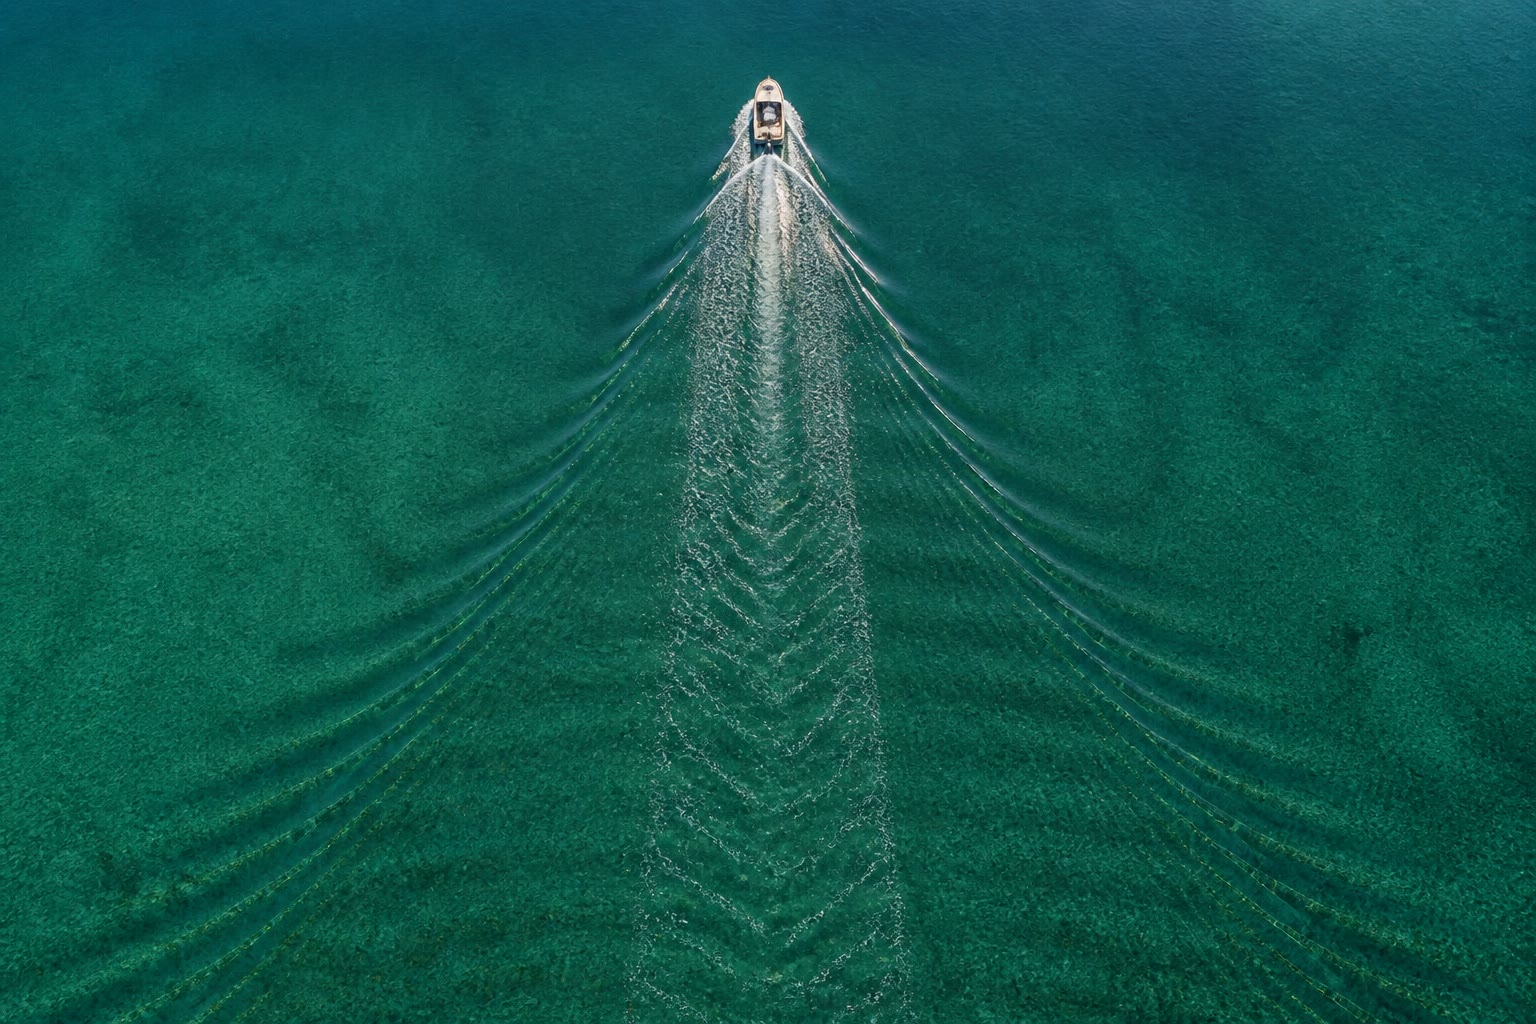
\includegraphics[width=0.56\linewidth]{images/book4/ai/b4-08-boat-wake-aerial.jpg}

{\small أثر زورق آلي على بحيرة ساكنة: يبقى النقش المريَّش داخل إسفين زاويته ثابتة لأن طاقة كل موجة مائية تنتقل بنصف سرعة ذراها --- أي التبدد مرئيًّا.}
\end{omfigure}


\begin{example}[كلاين--غوردون: أسرع من الضوء، ولا]\label{ex:b2:dispersion-wave-packets:superluminal}
من أجل $\omega^2 = \omega_c^2 + c^2k^2$: $v_\varphi = \omega/k$ و $v_g = c^2k/\omega$، ومنه
$v_\varphi v_g = c^2$: فتفوق \omterm{def:b2:dispersion-wave-packets:relation}{سرعة الطور} $c$ (وفي الأيونوسفير تمضي ذرى
موجة عند \qty{10}{MHz} أسرع من الضوء) لكن \omterm{prop:b2:dispersion-wave-packets:group}{سرعة
المجموعة}، وهي التي تحمل الإشارة، تبقى دونها. ولا تنقل \omterm{def:b2:dispersion-wave-packets:relation}{سرعة الطور}
طاقة ولا معلومة --- فالذرى كبقعة حزمة منارة
تكنس غيمة بعيدة.
\end{example}

\begin{remark}[التمدد]\label{rem:b2:dispersion-wave-packets:spreading}
رزمة عرضها المكاني $\Delta x$ تحوي أعدادًا موجية على مدى $\Delta k \sim
1/\Delta x$ (وهو تقابل فورييه، مسلَّم به)؛ وتختلف سرعات مجموعة
مركّباتها بالمقدار $\Delta v_g \approx |\omega''|\Delta k$، ومنه تكون بعد الزمن $t$ قد
تمددت بالمقدار $|\omega''|\Delta k\,t$: فيتضاعف عرضها بعد $t_{\text{تمدد}}
\sim \Delta x^2/|\omega''|$. ورزمة من عشر أمواج ماء عميق طولها \qty{100}{m}
($\Delta x \approx \qty{1}{km}$، و $\omega'' = -\tfrac14\sqrt{g/k^3} = \qty{-50}{m^2/s}$)
تتضاعف في نحو ست ساعات؛ ونبضة ضوء مدتها \qty{1}{ns} في
ليف بصري تتمدد بعشرات البيكوثانية في الكيلومتر --- وهو
حدّ معدل البتّات في الوصلات الطويلة. وتتمدد \omterm{prop:b2:dispersion-wave-packets:group}{الرزمة الموجية} الكمومية في
\cref{ch:b2:schrodinger-wave-functions} للسبب نفسه.
\end{remark}

\section{الكابل المحوري}

\begin{proposition}[معادلتا التلغراف؛ الخط عديم الضياع]\label{prop:b2:dispersion-wave-packets:coax}
\index{كابل محوري}\index{معادلتا التلغراف}\index{ممانعة مميزة}\index{خط نقل}
\omterm{prop:b2:dispersion-wave-packets:coax}{للكابل المحوري} (أو أي خط ذي ناقلين)، في واحدة الطول،
محارضة $\Lambda$ وسعة $\Gamma$. ويحقق التوتر $v(x, t)$ بين
الناقلين والتيار $i(x, t)$ في الداخلي منهما
\emph{معادلتي التلغراف}
\[
\frac{\partial v}{\partial x} = -\Lambda\frac{\partial i}{\partial t} , \qquad
\frac{\partial i}{\partial x} = -\Gamma\frac{\partial v}{\partial t} ,
\]
ومنهما \omterm{thm:b2:waves-on-strings:equation}{معادلة دالمبير} من أجل $v$ و $i$ مع
\[
c = \frac1{\sqrt{\Lambda\Gamma}} , \qquad
v = Z_c\,i \ \text{من أجل موجة نحو } +x, \quad Z_c = \sqrt{\frac\Lambda\Gamma} ,
\]
حيث $Z_c$ هي \emph{\omterm{prop:b2:dispersion-wave-packets:coax}{الممانعة المميزة}} للخط. ومن أجل
\omterm{prop:b2:dispersion-wave-packets:coax}{كابل محوري} نصفا قطريه $a < b$ ومملوء بعازل نفوذيته
النسبية $\varepsilon_r$، يكون $\Lambda = \dfrac{\mu_0}{2\pi}\ln\dfrac ba$، و $\Gamma =
\dfrac{2\pi\varepsilon_0\varepsilon_r}{\ln(b/a)}$، ومنه $c = c_0/\sqrt{\varepsilon_r}$ (أي نحو
\qty{2e8}{m/s}، ثلثا سرعة الضوء) و $Z_c = \dfrac{60\,\Omega}
{\sqrt{\varepsilon_r}}\ln\dfrac ba$: أي \qty{50}{\ohm} أو \qty{75}{\ohm} في الكابلات المعتادة.
\end{proposition}

\begin{proof}
نمذج الشريحة $[x, x + \dd x]$ بمحارضة على التسلسل $\Lambda\dd x$ وسعة
على التفرّع $\Gamma\dd x$: فيكون هبوط التوتر على امتداد الشريحة
$\Lambda\dd x\,\partial_ti$، والتيار الضائع في السعة $\Gamma\dd x
\,\partial_tv$. ثم نشتقّ تقاطعيًّا. ومن أجل $v = f(x - ct)$، تعطي المعادلة الأولى
$i = f(x - ct)/\Lambda c = v/\sqrt{\Lambda/\Gamma}$. وأما قيمتا $\Lambda$ و
$\Gamma$ فهما قيمتا المكثف الأسطواني والمحرِّض المحوري
المحسوبتان في كتاب السنة الأولى.
\end{proof}

\begin{omfigure}
\begin{tikzpicture}[font=\small]
  \begin{scope}
    \draw (0,0) to[L, l=$\Lambda\,\dd x$] (2.2,0) to[C, l=$\Gamma\,\dd x$] (2.2,-1.6);
    \draw (0,-1.6) -- (2.2,-1.6);
    \draw (2.2,0) -- (3.8,0); \draw (2.2,-1.6) -- (3.8,-1.6);
    \draw[->] (0.1,0.35) -- (0.7,0.35); \node[font=\footnotesize] at (0.4,0.6) {$i(x)$};
    \draw[->] (2.9,0.35) -- (3.5,0.35); \node[font=\footnotesize] at (3.2,0.6) {$i(x+\dd x)$};
    \node[font=\footnotesize] at (-0.3,-0.8) {$v(x)$}; \node[font=\footnotesize] at (4.6,-0.8) {$v(x+\dd x)$};
    \draw (-0.6,-0.2) -- (-0.6,-1.4); \draw[->] (-0.6,-1.4) -- (-0.6,-0.3);
    \node[font=\footnotesize] at (1.6,-2.3) {شريحة واحدة من الخط};
  \end{scope}
  \begin{scope}[xshift=8.4cm, yshift=-0.8cm]
    \draw[thick, fill=omExo!30] (0,0) circle (1.3);
    \draw[thick, fill=omDef!15] (0,0) circle (1.05);
    \draw[thick, fill=omThm!40] (0,0) circle (0.3);
    \draw[<->] (0,0) -- (30:0.3) node[pos=1.6, font=\footnotesize] {$a$};
    \draw[<->] (0,0) -- (-50:1.05) node[pos=0.6, right, font=\footnotesize] {$b$};
    \node[font=\footnotesize] at (0,1.65) {العازل $\varepsilon_r$، والضفيرة، واللبّ};
    \node[font=\footnotesize] at (0,-1.75) {$Z_c = \dfrac{60\,\Omega}{\sqrt{\varepsilon_r}}\ln\dfrac ba$};
  \end{scope}
\end{tikzpicture}

{\small على اليسار: الدارة المكافئة لشريحة $\dd x$ من خط
عديم الضياع --- محارضة على التسلسل وسعة على التفرّع --- ومنها تنتج
\omterm{prop:b2:dispersion-wave-packets:coax}{معادلتا التلغراف}. وعلى اليمين: \omterm{prop:b2:dispersion-wave-packets:coax}{كابل محوري} في مقطعه؛ ولا يتوقف
$\Lambda$ و $\Gamma$ فيه إلا على نسبة نصفي القطرين وعلى
العازل.}
\end{omfigure}

\begin{omfigure}
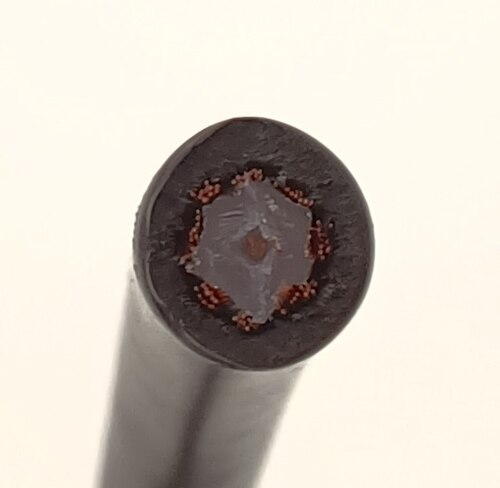
\includegraphics[width=0.46\linewidth]{images/book3/coaxial-cable.jpg}

{\small \omterm{prop:b2:dispersion-wave-packets:coax}{كابل محوري}: لبّ داخلي، وعازل، وناقل خارجي مضفور --- أي \omterm{prop:b2:dispersion-wave-packets:coax}{خط نقل} تحدّد محارضته وسعته في المتر سرعتَه وممانعتَه المميزة.}
\end{omfigure}

\begin{proposition}[الخط ذو الضياع؛ شرط انعدام التشويه]\label{prop:b2:dispersion-wave-packets:lossy}
\index{شرط هيفيسايد}\index{قانون كلفن في المربعات}
ومع مقاومة على التسلسل $R$ وموصولية على التفرّع $G$ في واحدة
الطول، تصير المعادلتان $\partial_xv = -\Lambda\partial_ti - Ri$ و $\partial_xi =
-\Gamma\partial_tv - Gv$، \omterm{def:b2:dispersion-wave-packets:relation}{وعلاقة التبدد} $\underline k^2 = (\Lambda\omega -
\iu R)(\Gamma\omega - \iu G)$: فالخط متبدّد وواهن. وله نهايتان:
(1) $R/\Lambda = G/\Gamma$ (وهو \omterm{prop:b2:dispersion-wave-packets:lossy}{شرط هيفيسايد}، ويُبلَغ بإضافة
محارضة): $\underline k = \omega\sqrt{\Lambda\Gamma} - \iu\sqrt{RG}$، فينتقل كل تواتر
بالسرعة نفسها وبالوهن نفسه --- فالخط \emph{يوهن} ولا
\emph{يشوّه}. (2) $\Lambda \approx 0$ و $G \approx 0$
(وهي حال أولى الكابلات البحرية): $\partial_x^2v = R\Gamma\,\partial_tv$، أي معادلة
\emph{انتشار} --- فلا تنتشر النبضة بل تنلطخ،
وتبلغ المسافة $L$ بعد زمن $\sim R\Gamma L^2$ (وهو قانون كلفن في
المربعات)، أي أطول بمئة مرة في كابل أطول بعشر مرات.
\end{proposition}

\begin{proof}
ندخل $\eu^{\iu(\omega t - kx)}$: $-\iu kv = -(\iu\omega\Lambda + R)i$، و $-\iu ki = -(\iu
\omega\Gamma + G)v$؛ ثم نضرب. وتحت \omterm{prop:b2:dispersion-wave-packets:lossy}{شرط هيفيسايد} يكون الجداء
مربعًا تامًّا. ونهاية الانتشار تسقط الحدّين $\iu\omega\Lambda$ و $G$.
\end{proof}

\begin{example}[ثلاثة كابلات]\label{ex:b2:dispersion-wave-packets:cables}
كابل الأطلسي سنة 1858: سلك نحاسي واحد في الغوتابركا،
و $R \approx \qty{3}{\ohm/km}$، و $\Gamma \approx \qty{0.3}{\micro F/km}$، و $L = \qty{3000}{km}$:
ومنه $R\Gamma = \qty{9e-10}{s/m^2}$ و $R\Gamma L^2 \approx \qty{8}{s}$ لكل نقطة: أي كلمة في
الدقيقة، وأتلفت محاولات المشغّلين فرضَ الإشارة
بتوتر \qty{2}{kV} العازلَ في أسابيع. وخط هاتفي
محمَّل بوشائع كل \qty{2}{km} تحقيقًا \omterm{prop:b2:dispersion-wave-packets:lossy}{لشرط هيفيسايد}
(سنة 1900): كلام واضح على مئات الكيلومترات. \omterm{prop:b2:dispersion-wave-packets:coax}{وكابل محوري} حديث عند \qty{50}{\ohm}:
$c = \qty{2e8}{m/s}$، و $\Lambda = \qty{0.25}{\micro H/m}$، و $\Gamma =
\qty{100}{pF/m}$، \omterm{def:b2:dispersion-wave-packets:complex}{ووهن}، سببه الأثر القشري في
الناقلين (\cref{ch:b2:waves-in-media})، ينمو مثل $\sqrt f$: أي بضعة
ديسيبلات في المئة متر عند \qty{100}{MHz}.
\end{example}

\begin{method}[قراءة علاقة تبدد]\label{met:b2:dispersion-wave-packets:method}
(1) اكتب معادلة أمواج الوسط بالترميز العقدي وحُلّها
بالنسبة إلى $\underline k(\omega)$. (2) وإذا كان $k$ حقيقيًّا: احسب $v_\varphi = \omega/k$ و
$v_g = \dd\omega/\dd k$ (أو $1/(\dd k/\dd\omega)$)؛ وقارن: أمتبدّد أم لا،
وأتبدّده عادي ($v_g < v_\varphi$) أم شاذّ. (3) وإذا كان $k$ عقديًّا: افصل
الانتشار ($k'$) عن \omterm{def:b2:dispersion-wave-packets:complex}{الوهن} ($k''$، وطوله $1/k''$)؛ والتخيلي الصرف
يعني \omterm{def:b2:dispersion-wave-packets:complex}{موجة متلاشية}، ولا نقل. (4) ويفصل تواتر القطع
حزمةً منتشرة عن حزمة متلاشية. (5) ومن أجل إشارة،
عوّل على الغلاف عند $v_g$، لا على الذرى أبدًا.
\end{method}

\section{تمارين}

\begin{exercise}[$\star$]\label{exo:b2:dispersion-wave-packets:1}
\omterm{ex:b2:dispersion-wave-packets:examples}{أمواج الماء العميق}، $\omega^2 = gk$. (أ) أوجد \omterm{def:b2:dispersion-wave-packets:relation}{سرعة الطور} \omterm{prop:b2:dispersion-wave-packets:group}{وسرعة المجموعة} و
دور موج طويل طوله \qty{100}{m}. (ب) وموج طويل دوره \qty{14}{s}:
أوجد طول الموجة و $v_\varphi$ و $v_g$؛ والزمن الذي تستغرقه طاقته في قطع \qty{5000}{km}.
(ج) ولماذا لا يصل إليها الموج القصير ذو الدور \qty{2}{s} أصلًا؟
\end{exercise}

\begin{exercise}[$\star$]\label{exo:b2:dispersion-wave-packets:2}
وسط يحقق $\omega^2 = \omega_c^2 + c^2k^2$ مع $\omega_c = 2\pi \times \qty{1e7}{rad/s}$
و $c = \qty{3e8}{m/s}$. ومن أجل $f = \qty{20}{MHz}$: أوجد $k$ و $v_\varphi$ و $v_g$ و
جداءهما. ومن أجل $f = \qty{5}{MHz}$: أوجد $\kappa$ وعمق النفوذ.
\end{exercise}

\begin{exercise}[$\star$]\label{exo:b2:dispersion-wave-packets:3}
شوكتان رنّانتان عند \qty{440}{Hz} و \qty{444}{Hz}: أوجد تواتر الضربات، و
دور تغيّرات العلوّ. وموجتان مائيتان طولاهما
\qty{100}{m} و \qty{110}{m}: أوجد تواتريهما، وطول موجة الغلاف وسرعته؛
وقارنها بالسرعة $v_g$ عند \qty{105}{m}.
\end{exercise}

\begin{exercise}[$\star$]\label{exo:b2:dispersion-wave-packets:4}
\omterm{prop:b2:dispersion-wave-packets:coax}{كابل محوري}: قطر ناقله الداخلي \qty{0.9}{mm}، والخارجي
\qty{3.0}{mm}، والبولي إيثيلين ($\varepsilon_r = 2.3$). أوجد $\Lambda$ و $\Gamma$ وسرعة الموجة،
\omterm{prop:b2:dispersion-wave-packets:coax}{والممانعة المميزة}، والتأخّر في المتر؛ وطول الكابل المكافئ
لتأخّر \qty{10}{ns}. والكابل نفسه بالهواء بدل البولي إيثيلين.
\end{exercise}

\begin{exercise}[$\star\star$]\label{exo:b2:dispersion-wave-packets:5}
\emph{الوتر الصلب.} يحقق وتر بيانو حقيقي $\mu\partial_t^2y = T\partial_x^2y
- EI\,\partial_x^4y$ (و $EI$ صلابة الانثناء). (أ) أوجد \omterm{def:b2:dispersion-wave-packets:relation}{علاقة التبدد}،
وسرعتي الطور والمجموعة. (ب) ومن أجل وتر لا$_4$ في
\cref{ch:b2:waves-on-strings} ($T = \qty{685}{N}$، و $\mu = \qty{6.1}{g/m}$، و $EI =
\qty{9.8e-3}{N.m^2}$)، أوجد الزيادة النسبية في $v_\varphi$ من أجل التوافقي
الثامن ($k = 8\pi/L$، و $L = \qty{0.38}{m}$)؛ وتحقق منها باللاتوافقية
الواردة هناك. (ج) وهل التبدد عادي أم شاذّ؟ وكيف تبدو قطفة
حادّة بعد بضع ذهابات وإيابات؟
\end{exercise}

\begin{exercise}[$\star\star$]\label{exo:b2:dispersion-wave-packets:6}
\emph{الوتر المتخامد.} $\mu\partial_t^2y + \alpha\partial_ty = T\partial_x^2y$. (أ) استنتج
\omterm{def:b2:dispersion-wave-packets:relation}{علاقة التبدد}. (ب) ومن أجل $\alpha \ll \mu\omega$، بيّن أن $k' \approx \omega/c$ و
$k'' \approx \alpha/2Z$؛ وأوجد \omterm{def:b2:dispersion-wave-packets:complex}{الوهن} \omterm{def:b2:sound-waves:decibel}{بالديسيبل} في المتر. (ج) والقيم: $\mu =
\qty{5}{g/m}$، و $T = \qty{50}{N}$، و $\alpha = \qty{0.02}{kg.m^{-1}.s^{-1}}$، و $f =
\qty{100}{Hz}$: تحقق من التقريب وأعطِ $\delta$. (د) وهل الوتر المتخامد
متبدّد؟ وفي أي نظام من $\alpha$ يصير كذلك؟
\end{exercise}

\begin{exercise}[$\star\star$]\label{exo:b2:dispersion-wave-packets:7}
\emph{التموّجات.} تحكم أمواجَ الماء القصيرة قوةُ \omterm{rem:b2:viscous-flows:capillarity}{التوتر السطحي}: $\omega^2 =
\gamma k^3/\rho$ (و $\gamma = \qty{0.072}{N/m}$)؛ والعلاقة الكاملة $\omega^2 = gk +
\gamma k^3/\rho$. (أ) أوجد $v_\varphi$ و $v_g$ للأمواج الشعرية الصرفة؛ وأيهما
أكبر؟ (ب) بيّن أن \omterm{def:b2:dispersion-wave-packets:relation}{سرعة الطور} في العلاقة الكاملة
أصغرية عند $\lambda_m = 2\pi\sqrt{\gamma/\rho g}$ واحسب $\lambda_m$ و $v_{\min}$.
(ج) وزورق أبطأ من $v_{\min}$ لا يترك أثرًا: فلماذا؟ (د) وقطرات المطر على
بركة تصنع حلقات تتخلف ذراها عن الحلقة: ففي أي نظام؟
\end{exercise}

\begin{exercise}[$\star\star$]\label{exo:b2:dispersion-wave-packets:8}
\emph{التمدد.} رزمة عرضها الابتدائي $\Delta x_0$ يتضاعف عرضها
بعد $t_{\text{تمدد}} \approx \Delta x_0^2/|\omega''(k_0)|$. (أ) مجموعة من \omterm{ex:b2:dispersion-wave-packets:examples}{أمواج
الماء العميق}، $\lambda = \qty{50}{m}$، و $\Delta x_0 = \qty{500}{m}$. (ب) ونبضة ضوء في
ليف زجاجي: $\omega'' \approx \qty{-0.16}{m^2/s}$؛ ونبضة مدتها \qty{10}{ps} ($\Delta x_0 =
\qty{2}{mm}$): أوجد زمن التمدد والمسافة المقطوعة في أثنائه؛ والأمر نفسه
من أجل نبضة \qty{1}{ns}. ولماذا تستعمل الوصلات البصرية الطويلة نبضات أطول أو
ليفًا يعوّض التبدد؟
\end{exercise}

\begin{exercise}[$\star\star$]\label{exo:b2:dispersion-wave-packets:9}
\emph{الكابل البحري.} $R = \qty{3}{\ohm/km}$، و $\Gamma = \qty{0.3}{\micro F/km}$،
و $\Lambda$ و $G$ مهمَلان. (أ) بيّن أن $v$ يحقق معادلة انتشار وأعطِ
انتشاريته. (ب) \omterm{def:b2:dispersion-wave-packets:relation}{علاقة التبدد} $\underline k(\omega)$؛ \omterm{def:b2:dispersion-wave-packets:relation}{وسرعة
الطور} وطول \omterm{def:b2:dispersion-wave-packets:complex}{الوهن} عند \qty{1}{Hz} وعند \qty{10}{Hz}. (ج)
والزمن الذي «تصل» فيه إشارة على \qty{3000}{km} ($\sim R\Gamma L^2$)؛ وعدد الكلمات في
الدقيقة. (د) وعلاج هيفيسايد: أوجد المحارضة في الكيلومتر اللازمة من أجل
$R/\Lambda = G/\Gamma$ إذا كان $G = \qty{1e-7}{S/km}$؛ ولماذا كان يصعب إضافتها؟
\end{exercise}

\begin{exercise}[$\star\star\star$]\label{exo:b2:dispersion-wave-packets:10}
\emph{الطاقة تنتقل \omterm{prop:b2:dispersion-wave-packets:group}{بسرعة المجموعة}.} وتر على مهاد مرن:
$\mu\partial_t^2y = T\partial_x^2y - Ky$، وموجته $y = A\cos(\omega t - kx)$ مع $\omega^2 =
\omega_c^2 + c^2k^2$. (أ) كثافة الطاقة $e = \tfrac12\mu(\partial_ty)^2 + \tfrac12T
(\partial_xy)^2 + \tfrac12Ky^2$ وتدفقها $\mathcal P = -T\partial_xy\,\partial_ty$: تحقق من
$\partial_te + \partial_x\mathcal P = 0$. (ب) أوجد المتوسطين الزمنيين $\langle e\rangle$ و
$\langle\mathcal P\rangle$ للموجة. (ج) بيّن أن $\langle\mathcal P\rangle/
\langle e\rangle = c^2k/\omega = v_g$، لا $v_\varphi$. (د) وماذا يحدث لتدفق
الطاقة دون تواتر القطع؟
\end{exercise}

\begin{exercise}[$\star\star\star$]\label{exo:b2:dispersion-wave-packets:11}
\emph{الموج الطويل والتسونامي.} أمواج الماء ذات طول الموجة $\lambda$ على عمق $h$
تحقق $\omega^2 = gk\tanh kh$ (مسلَّم بها). (أ) استعد نهايتي الماء العميق و
الماء الضحل ($kh \ll 1$)؛ وأوجد سرعة أمواج الماء الضحل؛ وهل هي
متبدّدة؟ (ب) وتسونامي طول موجته $\lambda = \qty{200}{km}$ على \qty{4}{km} من المحيط:
أي نهاية، وما السرعة والدور؛ وزمن قطع \qty{8000}{km}. (ج) وسعته
في عرض البحر \qty{0.5}{m}: أوجد الطاقة في واحدة طول الذروة
(وسلّم بأن $E = \tfrac12\rho gA^2$ في واحدة المساحة) من أجل جبهة طولها \qty{1000}{km}؛ وماذا
يحدث حين يهبط العمق إلى \qty{10}{m}، إذا انحفظ تدفق الطاقة $Ev_g$
(وهو قانون غرين، $A \propto h^{-1/4}$)؟ (د) وموج طويل طوله \qty{100}{m}
يصل شاطئًا: عند أي عمق يبدأ بالإحساس بالقاع،
ولماذا تصير ذراه موازية للشاطئ؟
\end{exercise}

\begin{exercise}[$\star\star\star$]\label{exo:b2:dispersion-wave-packets:12}
\emph{نبضة على خط.} كابل عند \qty{50}{\ohm} طوله $\ell = \qty{100}{m}$
($c = \qty{2e8}{m/s}$) يُغذَّى عند $x = 0$ من مولّد مقاومته
الداخلية \qty{50}{\ohm} وينتهي عند $x = \ell$ بحمل $R_L$. (أ) بيّن
أن موجة تصل النهاية تنعكس بمعامل التوتر
$r = (R_L - Z_c)/(R_L + Z_c)$ (اكتب $v$ و $i$ موجةً واردة
مع منعكسة وافرض قانون أوم في الحمل). (ب) أوجد القيم من أجل
$R_L = 50$ و $0$ و $\infty$ و \qty{150}{\ohm}. (ج) وتُرسل نبضة مدتها \qty{1}{ns} وتوترها \qty{1}{V}:
فما الذي يبيّنه راسم الاهتزاز عند المولّد، ومتى، من أجل كل
حمل؛ ولماذا تهمّ مقاومة المولّد \qty{50}{\ohm}. (د) ويعيد عيب في كابل
مدفون صدى بعد \qty{1.8}{\micro s}: فأين هو؟ (وهو قياس الانعكاس في
مجال الزمن.)
\end{exercise}

\section{مسألة: الكابل والبحر}

\begin{problem}[{مسألة نهاية الأسبوع --- التبدد في العمل: الكابل
التلغرافي الذي لطّخ النقاط، والموج الطويل الذي يعلن عاصفة،
والتسونامي الذي يعبر محيطًا، والرزمة التي تتمدد}]
\label{pb:b2:dispersion-wave-packets:1}

\medskip
\noindent\textbf{الجزء I --- الكابل التلغرافي.}
كابل الأطلسي سنة 1866: $R = \qty{2.0}{\ohm/km}$، و $\Gamma = \qty{0.25}{\micro F/km}$،
و $\Lambda = \qty{0.5}{mH/km}$، و $G$ مهمَل، وطوله $L = \qty{3500}{km}$.
\begin{enumerate}
  \item اكتب معادلتي التلغراف مع $R$ واستنتج
        \omterm{def:b2:dispersion-wave-packets:relation}{علاقة التبدد} $\underline k^2 = \Gamma\omega(\Lambda\omega - \iu R)$.
  \item وعند أي تواتر يساوي $\Lambda\omega$ المقدارَ $R$؟ استنتج أنه من أجل
        تواترات التلغراف (بضعة هرتزات) يكون الخط في
        النظام الانتشاري.
  \item وفي ذلك النظام، $\underline k = \sqrt{-\iu R\Gamma\omega}$: أعطِ $k'$ و $k''$
        (وتذكّر أن $\sqrt{-\iu} = (1 - \iu)/\sqrt2$)؛ \omterm{def:b2:dispersion-wave-packets:relation}{وسرعة الطور} وطول
        \omterm{def:b2:dispersion-wave-packets:complex}{الوهن} عند \qty{1}{Hz}؛ ثم عند \qty{4}{Hz}.
  \item \omterm{def:b2:dispersion-wave-packets:complex}{الوهن} \omterm{def:b2:sound-waves:decibel}{بالديسيبل} على الكابل كله عند \qty{1}{Hz} وعند
        \qty{4}{Hz}. وأي تواتر ينجو؟ وماذا يفعل ذلك بنقطة
        حادّة؟
  \item تقدير كلفن لزمن العبور، $R\Gamma L^2$؛ ومعدل الكابل
        العملي بالكلمات في الدقيقة إذا كانت الكلمة نحو
        $10$ نقاط وشرطات وكان على النقاط ألا تتراكب.
  \item واقترح هيفيسايد رفع $\Lambda$: فأي قيمة تجعل $\Lambda\omega = R$
        عند \qty{4}{Hz}، وما السرعة \omterm{def:b2:dispersion-wave-packets:complex}{والوهن} عندئذ
        (خذ $G = 0$، ومنه لا يمكن تحقيق الشرط $R/\Lambda = G/\Gamma$
        تمامًا --- فاستعمل العلاقة العامة عند ذلك التواتر)؟
  \item وليف بصري حديث يحمل \qty{1e10}{bit/s}: قارن ذلك
        بالسؤال 5، بقوى العشرة.
\end{enumerate}

\medskip
\noindent\textbf{الجزء II --- الموج الطويل.}
الماء العميق: $\omega^2 = gk$.
\begin{enumerate}[resume]
  \item \omterm{def:b2:dispersion-wave-packets:relation}{سرعة الطور} \omterm{prop:b2:dispersion-wave-packets:group}{وسرعة المجموعة} بدلالة الدور $T$.
  \item وعاصفة على بعد \qty{4000}{km} من ساحل تولّد أمواجًا أدوارها
        من \qty{6}{s} إلى \qty{18}{s}: أوجد زمن وصول كل من الطرفين؛
        ومدة حدث الموج الطويل.
  \item بيّن أن الدور الواصل إلى ساحل على البعد $D$ يحقق
        $1/T = gt/4\pi D$، و $t$ محسوب من العاصفة: فينمو $1/T$
        خطيًّا مع الزمن. وتسجّل عوّامة $T = \qty{16}{s}$ في يوم عند الظهر
        و $T = \qty{12}{s}$ بعد \qty{24}{h} بالضبط: أوجد بعد
        العاصفة.
  \item والطاقة في واحدة مساحة موج طويل سعته $A$ هي $\tfrac12\rho
        gA^2$؛ أوجد الاستطاعة العابرة لخط طوله \qty{1}{m} من الذروة، من أجل $A =
        \qty{1.5}{m}$ و $T = \qty{12}{s}$. (استعمل \omterm{prop:b2:dispersion-wave-packets:group}{سرعة المجموعة} --- ولماذا؟)
  \item ومزرعة طاقة موجية جبهتها \qty{1}{km} بمردود $30\%$:
        أوجد الاستطاعة الكهربائية؛ وقارنها بعنفة ريحية (\qty{3}{MW}).
  \item وزورق بسرعة \qty{5}{m/s} على ماء عميق يترك خلفه أثرًا ساكنًا:
        فأي طول موجة سرعة طوره تساوي سرعة الزورق
        فيتبعه؟ ولماذا يجرّ النقش على شكل V أضيق مما
        يوحي به انتشار الذرى نفسها
        (فكّر في $v_g = v_\varphi/2$)؟
  \item وإذ ترقب مجموعة من الموج الطويل من جرف، صف ما تفعله
        ذروة بعينها أثناء مرور المجموعة بعوّامة
        ثابتة؛ وكم ذروةً تحوي مجموعة مدتها
        \qty{2}{min} عند $T = \qty{12}{s}$، وكم «عمرًا» لذروة يمثّل ذلك؟
\end{enumerate}

\medskip
\noindent\textbf{الجزء III --- التسونامي.}
$\omega^2 = gk\tanh kh$؛ وعمق الهادئ $h = \qty{4.0}{km}$.
\begin{enumerate}[resume]
  \item يرفع زلزال رقعة من قاع البحر عرضها \qty{100}{km} بمقدار
        \qty{2}{m}؛ وللموجة $\lambda \approx \qty{200}{km}$: تحقق من أنها موجة
        ماء ضحل وأعطِ سرعتها ودورها وزمن
        بلوغها ساحلًا على بعد \qty{6000}{km}.
  \item وهل هي متبدّدة؟ قارنها بالموج الطويل في الجزء الثاني: أتصل
        قبل الموج الطويل أم بعده؟ وأيهما يصل نبضةً
        واحدة؟
  \item وارتفاعها في عرض البحر \qty{0.6}{m}: أوجد الطاقة في المتر المربع؛
        والطاقة الكلية لجبهة طولها \qty{500}{km} موزَّعة على طول
        موجة واحد؛ وقارنها بانفجار \qty{1}{Mt} (أي \qty{4.2e15}{J}).
  \item قانون غرين: أوجد الارتفاع حين يهبط العمق إلى \qty{20}{m} قرب
        الشاطئ (وتدفق الطاقة $\tfrac12\rho gA^2v_g$ محفوظ، و $v_g = \sqrt{gh}$)؛
        والسرعة وطول الموجة هناك؛ ولماذا تنحدر الموجة عندئذ
        وتنكسر كجدار.
  \item ولا تلحظ سفينة في عرض البحر مرور التسونامي: فلماذا؟
  \item وتسجّل مقاييس مدّ على بعد \qty{6000}{km} الموجةَ: فماذا يعطي
        زمن الانتقال، ولماذا تكون السرعة المقيسة أقل قليلًا
        من $\sqrt{gh}$ فوق محيط متغير العمق؟
\end{enumerate}

\medskip
\noindent\textbf{الجزء IV --- الرزمة المتمددة.}
\begin{enumerate}[resume]
  \item من أجل الماء العميق، احسب $\omega''(k) = \dd^2\omega/\dd k^2$ وقيمته
        من أجل $\lambda = \qty{100}{m}$.
  \item ورزمة من \qty{10}{} أمواج كهذه ($\Delta x_0 \approx \qty{1}{km}$)
        تُطلَق: أوجد زمن التمدد $\Delta x_0^2/|\omega''|$؛ والمسافة التي
        تقطعها الرزمة في أثنائه.
  \item واشرح بالكلام لماذا تتمدد رزمة طيفها أضيق
        (أي رتلها أطول) أبطأ، ولماذا لا يكاد تسونامي
        الجزء الثالث يتمدد أصلًا.
  \item والتقدير نفسه من أجل إلكترون طول موجته \qty{0.1}{nm}
        محصور في \qty{1}{nm}، مع $\omega = \hbar k^2/2m$ (و $\hbar =
        \qty{1.05e-34}{J.s}$، و $m = \qty{9.1e-31}{kg}$): أوجد زمن التمدد و
        المسافة المقطوعة --- وهو أول تماسّ مع \omterm{prop:b2:dispersion-wave-packets:group}{الرزمة الموجية}
        الكمومية في \cref{ch:b2:schrodinger-wave-functions}.
  \item لخّص في جدول: \omterm{def:b2:dispersion-wave-packets:relation}{علاقة التبدد} و $v_\varphi$ و $v_g$ من أجل الكابل
        والموج الطويل والتسونامي والإلكترون، وهل يمدّد
        الوسط أم يوهن فحسب.
\end{enumerate}
\end{problem}
